% \section{The advantages of combining resolution and precision}
% \label{sec:motivation}

% Traditional data reduction techniques work by truncating either the finest few resolution levels, or
% the last few low-ordered bits, but rarely both. In this section, we show that significant gain can
% be achieved through reducing both data resolution and precision. For each data set, we construct and
% compare four different streams, namely \emph{by level}, \emph{by bit plane}, \emph{by wavelet norm},
% and \emph{by magnitude}. The first three streams were introduced in
% Section~\ref{sec:common-static-streams}. The \emph{by magnitude} stream mimics a common data
% reduction scheme in the literature, in which the smaller-magnitude wavelet coefficients are removed.
% Correspondingly, in \emph{by magnitude}, the chunks are sorted by the sum of magnitude of their
% respective coefficients, and chunks of the same coefficient are streamed together. 

% We compare the four streams using three common quantities, namely the function itself, the
% function's histogram, and an isocontour. Every time a new chunk arrives, we reconstruct the function
% (using the inverse wavelet transform) on the original-resolution grid, and compute the
% root-mean-square error between this reconstructed function and the original function. For the other
% two quantities, the RMSE is replaced by relevant error metrics (see Section~\ref{sec:histogram}
% and~\ref{sec:isocontour} for detailed discussions of these error metrics).
% Figure~\ref{fig:motivation-rmse} shows the results. Note that in all plots, we remove all chunks
% containing purely leading zero bits, as such chunks tend to be compressed away in practice. 

% \begin{figure}[h]
%   \centering
% 	\subcaptionbox{RMSE, left: \emph{plasma}, right: \emph{turbulence}}{
%   {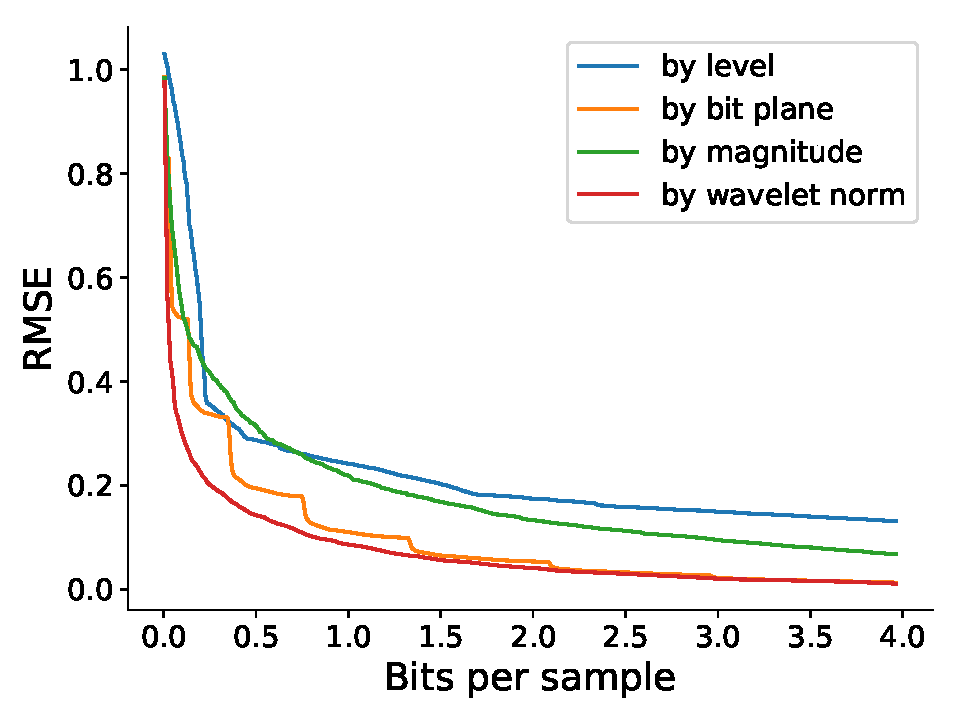
\includegraphics[width=0.48\linewidth]{img/motivation/motivation-psnr-plasma.pdf}}
%   {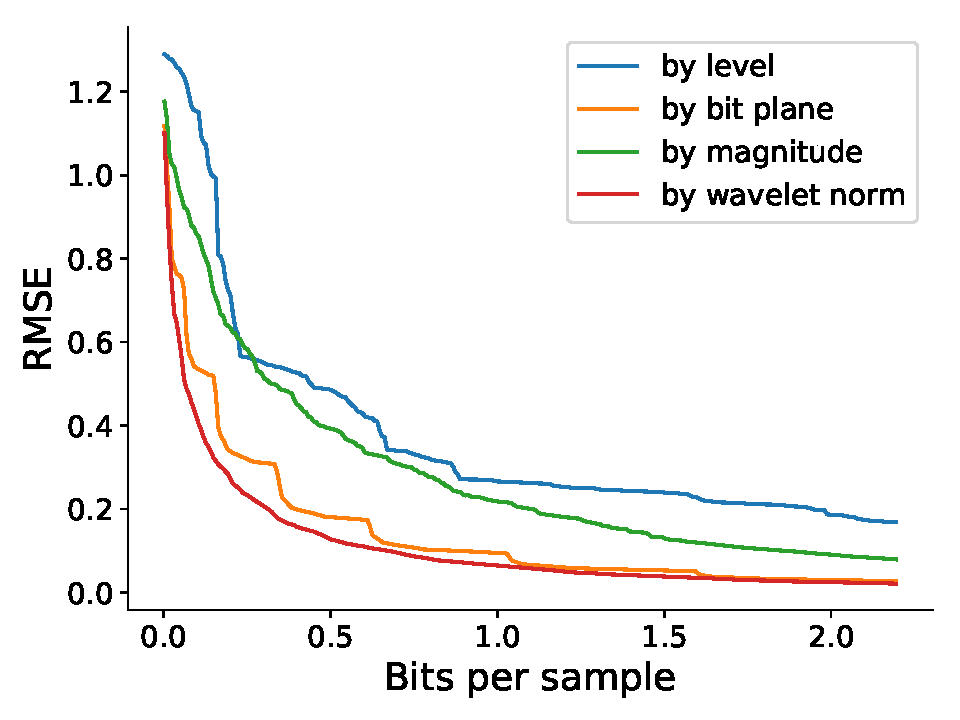
\includegraphics[width=0.48\linewidth]{img/motivation/motivation-psnr-turbulence.pdf}}}
%   \subcaptionbox{Histogram, left: \emph{plasma}, right: \emph{turbulence}}{
%   {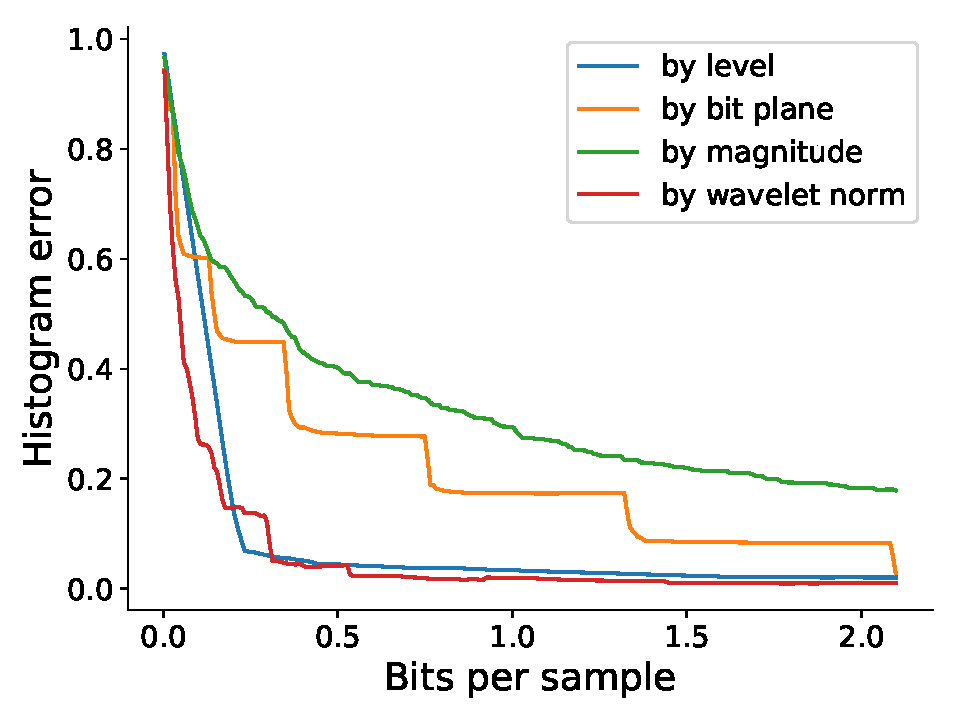
\includegraphics[width=0.48\linewidth]{img/motivation/motivation-histogram-plasma.pdf}}
%   {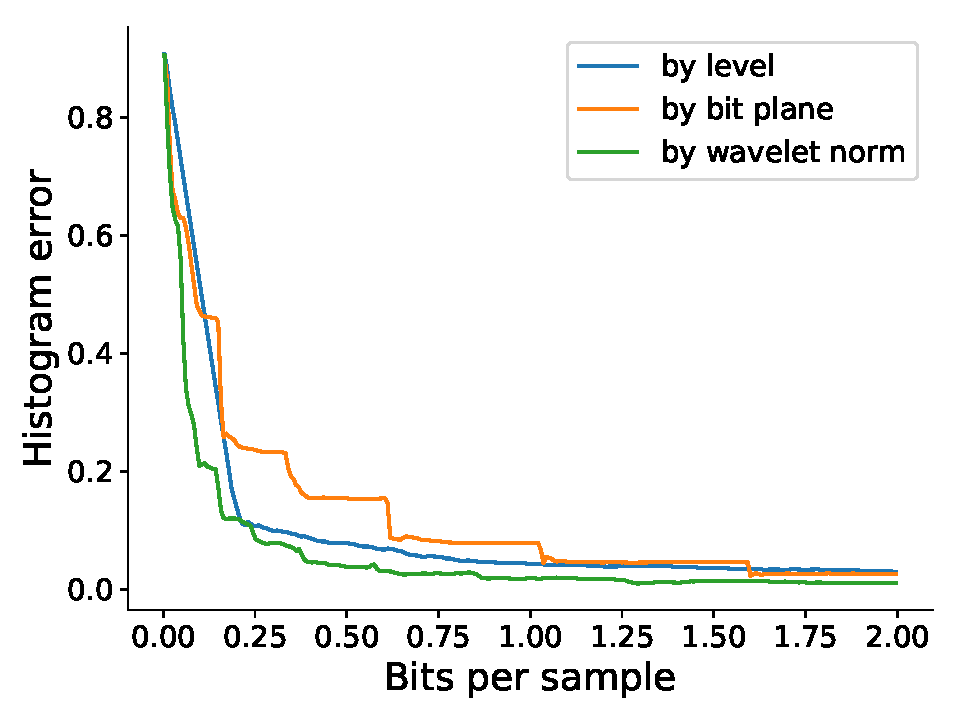
\includegraphics[width=0.48\linewidth]{img/motivation/motivation-histogram-turbulence.pdf}}}
%   \subcaptionbox{Isocontour, left: \emph{plasma}, right: \emph{turbulence}}{
%   {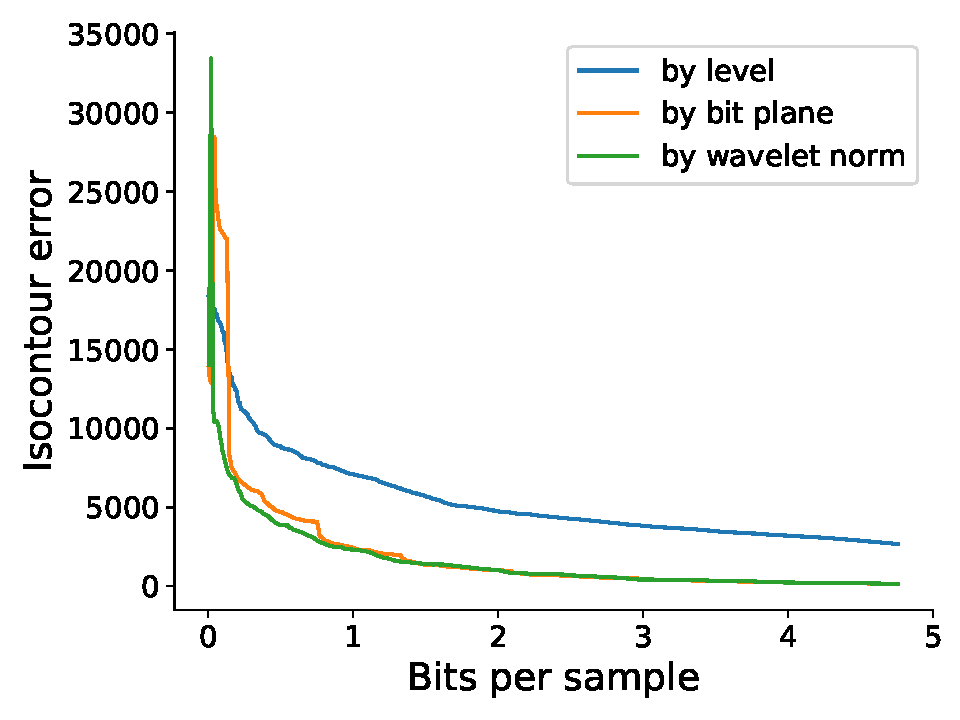
\includegraphics[width=0.48\linewidth]{img/motivation/motivation-isocontour-plasma.pdf}}
%   {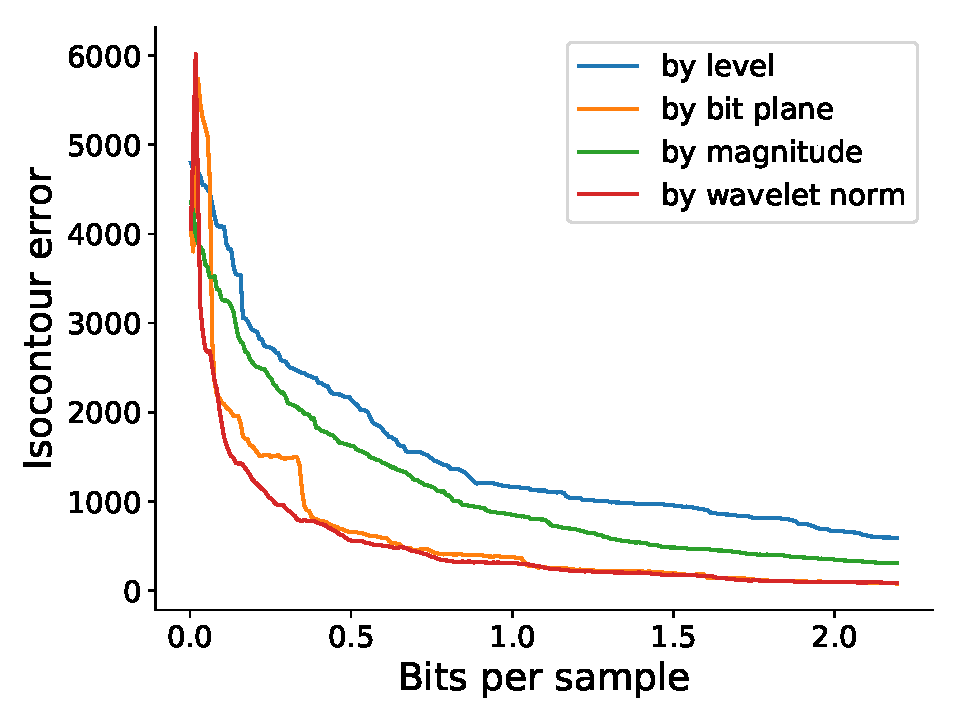
\includegraphics[width=0.48\linewidth]{img/motivation/motivation-isocontour-turbulence.pdf}}}
%   \caption{Comaprisons of the three static streams defined in Section \ref{sec:motivation}. Lower
%   error is better. The plots are truncated to better highlight the differences, without omitting
%   important information. Chunks containing leading zero bits are not plotted. In all cases, \emph{by
%   wavelet norm} performs the best.}
%  	\label{fig:motivation-rmse}
% \end{figure}

% The \emph{by wavelet norm} stream can be seen to consistently performs the best, across all data
% sets and quantities of interest. \emph{by bit plane} works almost as well as \emph{by wavelet norm}
% for function reconstruction and isocontour extraction, but not for histogram computation. The
% reverse is true for \emph{by level}. The \emph{by magnitude} stream performs somewhat better than
% \emph{by level}, except for histogram computation. Note that the our removal of leading zero bits
% penalizes the \emph{by level} stream more than it does the other streams, because in a typical data
% set, most leading-zero chunks exist in fine-resolution subbands (i.e., fine-scale coefficients tend
% to be smaller), which \emph{by level} only accesses later in the stream. The reason \emph{by wavelet
% norm} performs better than the rest is that a higher-ordered bit from a fine-scale coefficient might
% contribute more than a lower-ordered bit from a coarse-scale coefficient does (which \emph{by
% levell} is unable to take advantage of), and vice-versa (which \emph{by bit plane} ignores).

% The fact that \emph{by wavelet norm} outperforms all the other three suggests that performing data
% reduction in both resolution and precision can lead to significant quality improvements. In
% addition, it is possible that different analysis tasks require different types of streams for
% optimal results. This is hinted at by the fact that \emph{by level} underperforms \emph{by bit
% plane} for two of the three tasks, but outperforms it for the third (histogram). It seems likely,
% but uncertain at this point, whether \emph{by wavelet norm} is the best in all cases. To answer this
% question, we will expand our study to include dynamic streams that are optimized specifically for
% each quantity. While these data-dependent streams are unlikely to be realizable in practice, they
% can provide insights into designing practical data streams that improve on the generic \emph{by
% wavelet norm}, by being tailored to the analysis task at hand.

\section{Data-dependent, task-optimized streams}
\label{sec:data_dep_streams}

Each analysis task potentially requires a fundamentally different stream for optimal results. This
section aims to solve the problem of finding the most optimal stream possible, given a data set and
an error metric associated with the analysis task at hand. An error metric is a function
$E(Q(f'),Q(f))$ that returns the distance between its two arguments. $f$ is the original data field
and $f'$ is a reconstructed version of $f$ using a subset of the bits. $Q$ is a quantity of interest
(e.g., histogram, isocontour, etc) derived from $f$ or $f'$. There can be multiple error functions
$E$ that makes sense for the same $Q$. In this paper, we choose to use only one error metric with
each quantity, one which we believe is either common, or intuitive and simple while generalizable.
The list of quantity-optimized streams studied in this paper includes \emph{rmse-optimized} (Section
\ref{sec:rmse-optimized}), \emph{gradient-optimized} (Section \ref{sec:gradient}),
\emph{laplacian-optimized} (Section \ref{sec:laplacian}), \emph{histogram-optimized} (Section
\ref{sec:histogram}), and \emph{isocontour-optimized} (Section \ref{sec:isocontour}).

Studying a (data-dependent) quantity-optimized stream is important because such a stream serves both
as a benchmark, and a source of insights for other, more practical streams for the same quantity.
One way to define the ``optimal'' stream for a quantity $Q$ could be the stream that incurs the
minimum error $E$ at every point. However, in trying to realize it, our experience has been that
such a stream does not exist. Assume otherwise that the optimal stream exists, then by definition,
it must be possible to construct this stream using the following greedy algorithm: start with a pool
of all the chunks (and correspondingly an all-zero $f'$, and a presumably very high error $E$), pick
the chunk that when enabled, would minimize $E$, and remove it from the pool. Repeatedly pick and
remove the next chunk that minimizes $E$, until the pool is empty. This algorithm, however, can
encounter a situation in which the next chunk that minimizes the error is on a low-ordered bit plane
of a fine-scale coefficient, which contributes almost nothing to the reconstructed function. The
error is minimized because it is kept approximately constant. In this case it is actually better to
pick a chunk that increases the error slightly, but otherwise contributes a lot more to the
function. In optimization terms, it is necessary to move in a direction that increases the error to
avoid getting stuck in a local minima.

The optimal stream for an error metric can also be defined as the stream such that the area bounded
by its plotted error curve and the horizontal axis is the smallest. However, the usefulness of such
a definition is limited in practice, because a stream should be able to be terminated at any point
and still be expected to produce an error as small as possible. Therefore, instead of using this
definition of ``optimality'', we slightly modify the greedy algorithm stated above to avoid the
problem of being stuck in local minima. We start with a pool consisting of all the chunks and an
empty stream, and build this stream back-to-front. In particular, in each step, the chunk whose
removal from the pool has the least impact on the error $E$ is removed and inserted to the beginning
of the current stream. This algorithm solves the problem of unimportant chunks being picked too
early in the original algorithm, because here, chunks being picked early are at the end of the
stream, not the beginning.

In our experiments, however, this back-to-front greedy algorithm is too costly in practice. Ignoring
all the steps done in each iteration, this algorithm amounts to a 2-level nested loop running for
$n^2$ iterations, where $n$ is the number of chunks. In 2D, with a $256^2$ data set, a chunk size
that spans $16$ coefficients, and $16$ bits of quantization, $n^2$ would be in the billions, which
we have found to be prohibitively large. We have therefore adopted a simplified version of this
algorithm, where only one pass through the set of $n$ chunks is needed, reducing the number of
iterations from $n^2$ to $n$. The modified algorithm works as follows. We disable (sets to zero) a
new chunk $c_i$ in iteration $i$, then compute and record the error $E_i$ due to chunk $c_i$
missing, and enables $c_i$ again at the end of iteration $i$. After repeating the same process for
$n$ iterations, each chunk now has an associated weight, $E_i$. The optimal stream, then, is simply
a sorted list of chunks, in decreasing order of the weights. We have observed that this simplified
algorithm brings the running time down from days to minutes, while retaining the same quality of the
output stream. The pseudocode of the algorithm is presented in Algorithm~\ref{alg:greedy}.

\begin{algorithm}[h]
  \caption{Computing a task-optimized stream}
  \begin{algorithmic}[1]
    \Inputs{
			An original function $f$\\
			An unordered set of $n$ chunks $C = \{c_i\}, i\in \{0,\dots,n-1\}$\\
			A quantity of interest $Q$, and a distance function $E$}
		\Initialize{A set of weights $\Gamma = \{\gamma_i\}, i\in \{0,\dots,n-1\}$ }
		\For{each chunk $c_i$}
			\State $c_i \gets 0$
      \State Back-transform $C$ to produce a set of wavelet coefficients $W$
			\State Perform inverse wavelet transform on $W$ to produce $f'$
			\State $\gamma_i \gets E(Q(f'),Q(f))$			
			\State Restore $c_i$
		\EndFor
		\State Sort the $c_i$'s in descending order of $\gamma_i$.
		\Output{The $Q$-optimized stream, which is the sorted $C$}
	\end{algorithmic}
	\label{alg:greedy}
\end{algorithm}
